\subsection{支持向量回归（SVR）}
\label{sec:regression-svr}

分位数损失对低估和高估分别固定不对称的代价；Huber损失在中部平方、尾部线性，但只要偏离就计分。\term{支持向量回归}（support vector regression, SVR）再进一步：允许预测落在一个宽度为$2\epsilon$的容忍带内而不计任何误差，只有超出带外的部分才受罚。这与“与预测完全一致才算拟合好”的思路不同：带内误差被视为可接受的精度余量，模型只对超出精度要求的偏差负责。Smola与Schölkopf在2004年给出SVR的系统算法综述\scite{smola2004svr}。

\subsubsection{模型结构}
\label{sec:regression-svr-structure}

线性预测仍为$f(\bm{x})=b+\bm{w}^{\top}\bm{x}$。定义$\epsilon$不敏感损失
\begin{equation}
  |e|_\epsilon=\max(0,|e|-\epsilon),
  \qquad e=y-f(\bm{x}),
  \label{eq:regression-svr-objective}
\end{equation}
即残差绝对值不超过$\epsilon$时损失为零，超出部分按线性累加。$\epsilon$是预先给定的容忍带半宽，$C>0$权衡拟合误差与参数幅度。图\ref{fig:regression-svr-objective}画出该损失：零点附近一段水平，两侧斜率为1。

\begin{figure}[htbp]
  \centering
  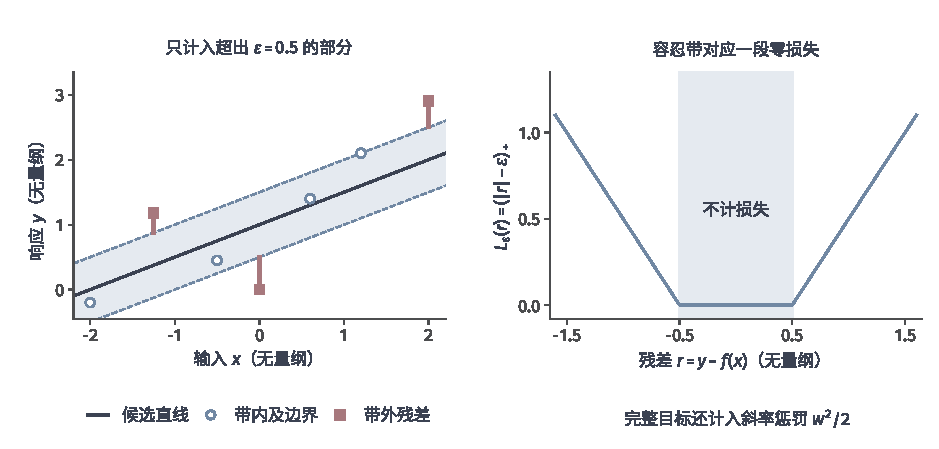
\includegraphics[width=105.412mm]{figures/04-classic-models/00-shared/matplotlib/regression-svr-objective/figure.pdf}
  \caption{$\epsilon$不敏感损失（$\epsilon=0.5$）。残差$|e|\leq0.5$时损失为零，超出部分按线性增长；水平段对应预测允许的精度余量，两侧斜线对应带外惩罚。}
  \label{fig:regression-svr-objective}
\end{figure}

把带外偏差拆为上、下两个非负松弛$\xi_i,\xi_i^\star\geq0$，原始目标为
\begin{equation}
  \min_{b,\bm{w},\xi,\xi^\star}
  \frac12\lVert\bm{w}\rVert_2^2
  +\frac{C}{n}\sum_{i=1}^n(\xi_i+\xi_i^\star),
  \label{eq:regression-svr-primal}
\end{equation}
约束为
\[
  y_i-b-\bm{w}^{\top}\bm{x}_i\leq\epsilon+\xi_i,\quad
  b+\bm{w}^{\top}\bm{x}_i-y_i\leq\epsilon+\xi_i^\star,\quad
  \xi_i,\xi_i^\star\geq0.
\]
目标凸、约束线性，是凸二次规划。二次项惩罚参数幅度，线性项只计带外偏差，两者分工明确；截距与强度的归一化约定与其他带惩罚模型一致。

\subsubsection{参数学习}
\label{sec:regression-svr-learning}

\paragraph{对偶目标的推导}

对上、下约束分别引入乘子$\alpha_i\geq0$、$\alpha_i^\star\geq0$，写出拉格朗日函数。对$b$求导得$\sum_i(\alpha_i-\alpha_i^\star)=0$；对$\bm{w}$求导并令其为零，得
\begin{equation}
  \bm{w}=\sum_{i=1}^n(\alpha_i-\alpha_i^\star)\bm{x}_i.
  \label{eq:regression-svr-dual-w}
\end{equation}
把这一关系代回拉格朗日函数，消去$\bm{w}$与松弛变量，得到对偶目标
\begin{equation}
  \max_{\alpha,\alpha^\star}
  -\frac12\sum_{i,j}(\alpha_i-\alpha_i^\star)
    (\alpha_j-\alpha_j^\star)\bm{x}_i^{\top}\bm{x}_j
  -\epsilon\sum_i(\alpha_i+\alpha_i^\star)
  +\sum_i y_i(\alpha_i-\alpha_i^\star),
  \label{eq:regression-svr-dual}
\end{equation}
约束为$0\leq\alpha_i,\alpha_i^\star\leq C/n$与$\sum_i(\alpha_i-\alpha_i^\star)=0$。当前凸问题满足强对偶条件，数据内积只以$\bm{x}_i^{\top}\bm{x}_j$的形式出现，这为后面替换核内积留出了位置；接下来需要学习的就是这些盒约束乘子。

\paragraph{数值求解与参数恢复}

对偶是盒约束二次规划，全规模解法存储与运算量约为$O(n^2)$。工程上采用分解方法：保持等式和盒约束，每轮只更新少量乘子组成的工作集，保持其余乘子可行，在当前可行初值上使目标上升；最优性检查由KKT违反程度决定，达到容差或迭代预算即停。由最优乘子按式\eqref{eq:regression-svr-dual-w}恢复$\bm{w}$；若存在满足$0<\alpha_i<C/n$或$0<\alpha_i^\star<C/n$的内点乘子，由对应约束等式求$b$；没有内点时，按KKT条件在可行区间内取一个$b$。新输入预测为
\[
  f(\bm{x}_\star)=b+\sum_{i=1}^n(\alpha_i-\alpha_i^\star)\bm{x}_i^{\top}\bm{x}_\star.
\]

\subsubsection{理论分析}
\label{sec:regression-svr-theory}

\paragraph{支持样本与容忍带}

\begin{lemma}[SVR的支持样本]
\label{lem:regression-svr-support}
在凸SVR问题中，只有违反容忍带或恰在带边界上的样本可能有非零乘子：当$|y_i-f(\bm{x}_i)|<\epsilon$时$\alpha_i=\alpha_i^\star=0$。带内样本不进入式\eqref{eq:regression-svr-dual-w}的参数与预测；边界样本的非零乘子有两种情形，由该样本落在上边界还是下边界决定。
\end{lemma}

\begin{proof}
由KKT互补松弛，乘子为正要求对应松弛或约束取等。带内样本两条约束都严格成立、松弛为零，故乘子必须为零；参数只由带外与边界样本——\term{支持向量}（support vectors）——决定，预测求和也只遍历它们。非零乘子蕴含对应残差条件，反向却未必成立；零带宽$\epsilon=0$时退化为对所有样本计分的情形。
\end{proof}

\paragraph{最优性与预测含义}

二次项$\lVert\bm{w}\rVert_2^2/2$严格凸，故$\bm{w}$唯一；$b$在没有内点乘子时可在可行区间内取值，不必唯一。训练成本随$n$平方增长，预测只走支持样本，支持样本越少预测越省。该损失一般不等于条件均值或指定分位数目标。与岭回归对照：岭用二次惩罚连续收缩全部系数，SVR用$\epsilon$带让多数样本乘子归零，两者都是带惩罚的凸拟合，但稀疏性来自容忍带而非一范数。

\paragraph{支持非线性关系：核SVR}
\label{sec:regression-kernel-svr}

把原始内积$\bm{x}_i^{\top}\bm{x}_j$换成核$k(\bm{x}_i,\bm{x}_j)$，线性SVR就在再生核希尔伯特空间（RKHS）中工作。RKHS内积由核给出
\begin{equation}
  \langle\phi(\bm{x}_i),\phi(\bm{x}_j)\rangle_{\mathcal H}=k(\bm{x}_i,\bm{x}_j),
  \label{eq:regression-rkhs-inner-product}
\end{equation}
并满足再生性：对任意$f\in\mathcal H$，$f(\bm{x})=\langle f,\phi(\bm{x})\rangle_{\mathcal H}$，即函数在$\bm{x}$处的值等于它与该点特征内积。二次项$\lVert\bm{w}\rVert_2^2/2$对应RKHS范数惩罚，限制函数大小；对偶目标只需把数据内积替换为Gram矩阵$\bm{K}$的元素$k_{ij}$，预测变为
\begin{equation}
  f(\bm{x}_\star)
  =b+\sum_{i\in\mathrm{SV}}(\alpha_i-\alpha_i^\star)k(\bm{x}_i,\bm{x}_\star).
  \label{eq:regression-kernel-svr-prediction}
\end{equation}
核的合法性与常用形式见第\ref{sec:classic-overview-kernel-validity}节和第\ref{sec:classic-overview-common-kernels}节。训练仍解式\eqref{eq:regression-svr-dual}的盒约束二次规划，只需更换Gram矩阵；核、$C$与$\epsilon$一起由训练内验证选择，比较训练存储与支持样本预测代价时不必依赖后文显式基函数的展开。
